\documentclass{article}


% if you need to pass options to natbib, use, e.g.:
%     \PassOptionsToPackage{numbers, compress}{natbib}
% before loading neurips_2024

\PassOptionsToPackage{numbers, compress}{natbib}

% ready for submission
%\usepackage{neurips_2024}
\bibliographystyle{abbrvnat}

\usepackage[pdftex]{graphicx}

% to compile a preprint version, e.g., for submission to arXiv, add add the
% [preprint] option:
%\usepackage[preprint]{neurips_2024}


% to compile a camera-ready version, add the [final] option, e.g.:
\usepackage[final]{neurips_2024}




\usepackage[utf8]{inputenc} % allow utf-8 input
\usepackage[T1]{fontenc}    % use 8-bit T1 fonts
\usepackage{hyperref}       % hyperlinks
\usepackage{url}            % simple URL typesetting
\usepackage{booktabs}       % professional-quality tables
\usepackage{amsfonts}       % blackboard math symbols
\usepackage{amsmath}
\usepackage{nicefrac}       % compact symbols for 1/2, etc.
\usepackage{microtype}      % microtypography
\usepackage{xcolor}         % colors


\title{SmokeViz: Using Pseudo-Labels to Develop a Deep Learning Dataset of Wildfire Smoke Plumes in Satellite Imagery}


% The \author macro works with any number of authors. There are two commands
% used to separate the names and addresses of multiple authors: \And and \AND.
%
% Using \And between authors leaves it to LaTeX to determine where to break the
% lines. Using \AND forces a line break at that point. So, if LaTeX puts 3 of 4
% authors names on the first line, and the last on the second line, try using
% \AND instead of \And before the third author name.


\author{%
    Rey Koki\(^{1,2}\)  \thanks{corresponding author: \texttt{rey.koki@colorado.edu} } \quad Michael McCabe\(^{1}\) \quad Dhruv Kedar\(^{1}\)\\ 
    \textbf{Christina Kumler-Bonfanti}\(^{1,2}\) \quad \textbf{Jebb Stewart}\(^{2}\) \quad  \textbf{Jed Brown}\(^{1}\) \\
    \(^1\)University of Colorado, Boulder \quad \(^2\)National Oceanic and Atmospheric Administration\\
}
  % Affiliation \\
  % Address \\
  % \texttt{email} \\
  % \AND
  % Coauthor \\
  % Affiliation \\
  % Address \\
  % \texttt{email} \\
  % \And
  % Coauthor \\
  % Affiliation \\
  % Address \\
  % \texttt{email} \\
  % \And
  % Coauthor \\
  % Affiliation \\
  % Address \\
  % \texttt{email} \\


\begin{document}


\maketitle


\begin{abstract}
The increase in the frequency of wildfires on a global scale underscores the need for advancements in fire monitoring techniques for disaster management, environmental protection and to mitigate negative health outcomes. This research introduces an innovative, data-driven framework that leverages the semi-supervised method, pseudo-labeling, to generate smoke plume annotations in geostationary satellite imagery. Unlike many pseudo-labeling applications that aim to increase the labeled dataset size, the primary objective is use pseudo-labels to refine an existing National Oceanic and Atmospheric Administration smoke dataset that provides temporal and geographical information on individual smoke plumes but at variable and, primarily, low temporal resolution. We use deep learning and pseudo-labels to pinpoint the singular, most representative, satellite image that optimally illustrates the smoke annotation within the given time window. By identifying the most representative imagery of smoke plumes for a given smoke annotation, the study seeks to create an accurate and relevant machine learning dataset. The resulting dataset is anticipated to be an instrumental tool in developing further machine learning models, such as an automated system capable of real-time monitoring and annotation of smoke plumes directly from streaming satellite imagery.
\end{abstract}


\section{Introduction}

In recent years, the escalation of wildfire incidents worldwide has become a prominent environmental and public health concern. The combustion process in wildfires releases smoke containing fine particulate matter (PM2.5) and harmful gases, posing severe hazards to human health and air quality. These risks underscore the necessity for efficient and effective monitoring methods to mitigate the adverse health impacts associated with wildfire smoke. 

Traditionally, wildfire monitoring has relied on ground-based methods, such as forest service patrols, manned lookout towers, and aviation surveillance \cite{smoke_monitoring}. While these methods provide valuable localized insights, they are constrained by geographical and logistical limitations, often failing to deliver timely and comprehensive data, especially over large and remote areas. In contrast, satellite imagery offers a vantage point that overcomes these limitations, providing continuous, wide-area coverage and real-time data crucial for assessing and responding to the health risks posed by wildfire smoke.

Satellite imagery, equipped with state-of-the-art sensors, such as the Advanced Baseline Imager (ABI) on the Geostationary Operational Environmental Satellites (GOES) \cite{goes}, have revolutionized environmental monitoring. These tools enable the detailed observation of smoke plumes, their particulate density, and the extent of smoke spread. These satellite-based systems offer the capabilities to provide critical insights into the concentration and movement of smoke particulates, facilitating real-time assessments of air quality.

The integration of satellite imagery in wildfire smoke monitoring is not only instrumental in providing real-time data but also plays a significant role in public health planning and response. By mapping the spread and density of smoke, health authorities can issue timely warnings, implement evacuation protocols, and deploy resources effectively to mitigate health risks. Furthermore, long-term data gathered from satellite observations can aid in understanding the broader impacts of wildfire smoke on public health, influencing policy decisions and preventive measures.

Currently, multi-channel thresholding is a popular method to distinguish smoke pixels from pixels containing dust, clouds or other phenomenon with similar signatures \cite{threshold}. Thresholds are determined by using historical, labeled data to extract optimal radiance values for each channel that corresponds with the labeled class. These methods are tuned to particular biogeographies and often have issues with generalization to new locations with varying fuel types \cite{thresh_geog}.

In contrast to the numerical thresholding approach, human visual inspection of satellite imagery is another commonly used method for smoke identification. Trained analyst inspect satellite imagery and label the smoke by hand. An example of hand-labeled annotations is the National Oceanic and Atmospheric Administration (NOAA) Hazard Mapping System (HMS) fire and smoke product \cite{hms, hms_val}. For the HMS smoke product, trained satellite analysts use movement characteristics to help identify smoke by scanning through a time series of satellite imagery. When visual inspection indicates smoke, the analyst will draw a polygon that corresponds to the geolocation and density of smoke. By design of the product, the HMS annotations have varying time resolution and are released on a rolling but undefined schedule ranging from one to multiple times a day as observation conditions permit. This method is potentially not as scalable as an automated approach and is limited by the availability of analysts and their time. 

To address the challenges associated with thresholding and manual labels, we can look towards innovative approaches and recent technological advancements in computer vision. Machine learning methods have shown potential in improving the accuracy and efficiency of satellite-based wildfire smoke detection and monitoring. For instance, SmokeNet, uses a convolutional neural network (CNN) based framework to determine if a scene of MODIS satellite imagery contains smoke \cite{smokenet}. Another study, that looked at a singular wildfire event, also used a CNN to identify smoke on a pixel-wise basis using imagery from Himiwari-8 \cite{larsen}. Additionally, Wen et al. developed a CNN architecture that takes GOES-East imagery as input and the HMS-generated annotations for the target labels during training \cite{smoke_goes}. 

The success of deep learning methods, such as CNNs, relies heavily on the availability of a large, representative dataset \cite{data_size}. As laid out in table \ref{studies}, prior studies use relatively small numbers of samples, from 47 \cite{wang} to 6825 \cite{smoke_goes}, where one sample represents a satellite image with a singular time and geolocation. In contrast, benchmark datasets for image classification contain tens of thousands (CIFAR-10 and MNIST) to millions (CIFAR-100 and ImageNet) of data samples \cite{cifar}, \cite{mnist}, \cite{imgnet}. Keeping in mind the correlation between both the quality and quantity of data with model performance, we introduce the largest known smoke dataset, SmokeViz, containing over 130,000 samples.

\begin{table}[h]
    \caption{Comparison of different studies including method used, dataset size, satellite source, number of channels used and if classification is performed at a pixel or image level.}\label{studies}
    \centering
    \begin{tabular}{ccccrrcrc}
        \toprule
        Reference & Method & \verb|#| Samples & Satellite & \verb|#| Channels & Level\\
        \midrule
        \cite{smokenet}& CNN & 6255 & MODIS & 5 & image\\
        \cite{smoke_goes}& CNN & 6825 & GOES-East & 5 & pixel\\
        \cite{larsen} & CNN & 975 & Himiwari-8 & 7 & pixel\\
        \cite{wang}& U-Net & 47 & Landsat-8 & 13 & pixel\\
        SmokeViz  & U-Net & 133,871 & GOES-East/West & 3 & pixel\\
        \bottomrule
    \end{tabular}
\end{table}


Semi-supervised learning is an approach that can be used to increase the number of labeled samples in a dataset. This is done by leveraging a labeled dataset to generate new labels for an often larger, but unlabeled, dataset. Pseudo-labeling, a form of semi-supervised learning, uses labeled data to train an initial model, then runs that model on unlabeled data to predict pseudo-labels, and finally trains a new model using the pseudo-labels \cite{pseudo}. We introduce a variation of pseudo-labeling, not to increase the size, but to increase the quality of our dataset by generating pseudo-labels to select the best satellite image out of a given time-window to represent each smoke plume annotation.


\section{Methods}
\subsection*{Dataset}

The initial source for smoke labels, discussed in further detail in the HMS Smoke Labels section, is uniquely characterized by each annotation, \(y\), having corresponding imagery ranging between 1-60 frames, where each frame, \(x\), captures 5 minutes of exposure. Additionally, we have two satellites that overlap in coverage area, GOES-East and GOES-West, effectively doubling the number of frames for a single annotation. For the set of smoke annotations, \(\mathcal{Y}\), \(y \in \mathcal{Y}\) uses one or more \(x \in \mathcal{X}\) where \(\mathcal{X}\) is the entire set of satellite imagery corresponding to the set of time windows defined by the labels. We apply pseudo-labeling to develop a subset of \(\mathcal{X}\), denoted as \(\mathcal{X}_p\), that has a one-to-one annotation-to-image ratio such that \(|\mathcal{X}_p| = |\mathcal{Y}|\), where we choose the satellite image that has the maximum overlap between the geolocation of smoke in the imagery and the analyst annotation.

Dataset development came in three stages. First, we create an initial dataset, \(\mathcal{X}_M\), that leverages light scattering physics to determine which singular satellite image would be in the optimal configuration for smoke detection. Second, we used \(\mathcal{X}_M\) to train an initial parent model, \(f_{\circ}\), that identifies smoke in satellite imagery. Third, we use \(f_{\circ}\) to label each satellite image in a given annotation's time-window and the optimal satellite image is chosen based on which image's pseudo-labels has the greatest overlap with the analyst annotation for the given location and densities of smoke.

\subsubsection*{HMS Smoke Labels} 
NOAA manages environmental satellite programs such as the HMS program, the HMS program is an operational system that uses an aggregation of satellite data to generate active fire and smoke data. To train our model, we implement a supervised learning framework that uses the HMS analyst smoke product as truth labels during the model training process.

HMS smoke analysis data gives the coordinates of the smoke perimeter as a polygon and classifies the smoke by density within a given time window. The time windows can range from instantaneous (same start and end time) to lengths of 5 hours. While the true bounds of the smoke can change within the larger time spans, the analyst is making an approximation that should reflect the smoke coverage over the duration of the time window. The density information is qualitatively determined by each analyst based on the apparent smoke opacity in the satellite imagery and categorized as either light, medium or heavy as seen in figure \ref{densities}a \cite{hms_web}.

\begin{figure}
    \centering
    \includegraphics[width=14cm]{figures/Misclassified.png}
    \caption{Satellite imagery captured by GOES-East within a few days of each other. The yellow, orange and red contours indicate the extent of Light, Medium and Heavy smoke. a) shows a canonical example of a smoke plume. b) and c) show observable variations in the density labels.}\label{densities}
\end{figure}

\subsubsection*{Thermometer Encoding Smoke Densities}

One of the challenges introduced with using human generated qualitative smoke densities was that, as seen in figure \ref{densities}b and \ref{densities}c, there are variations in what is labeled as heavy or light density smoke. More generally, reproducing qualitative metrics with quantitative algorithms is a challenging problem, but we apply mathematical approaches that mitigate some of the underlying complications of our specific problem. Despite the fact that the smoke densities introduce qualitative complexities, we decided that the density approximations were important to use in our dataset because of the differences in signatures the densities produce. Within the satellite imagery, the appearance of a light density smoke plume will look significantly different than a heavy density smoke plume as seen in figure \ref{densities}. Additionally, a light density smoke plume is expected to be more challenging to detect since it is easier for it to be misclassified as not smoke. During the training process, the separate density categories allows us to deferentially weight the penalization given to the model for incorrect classifications based on category. For example, the model can be given a small penalization for misclassifying light smoke as not smoke while given a higher penalization for misclassifying heavy smoke as not smoke. 

In addition to the densities being ordered and categorical, the differences between the density categories are not evenly distributed by a given metric, such as particulate matter per square meter. The intervals between densities being unknown along with the hierarchical nature of the density labels makes the labels ordinal instead of just categorical. This data property allows us to use thermometer encoding \cite{therm_enc}, which leverages the idea that heavy density smoke includes both medium and light density smoke, that heavy density smoke is closer to medium than it is to light, and automatically weights the loss functions and incorporates the ranked ordering of the densities. As seen in Table \ref{therm}, one-hot encoding, commonly used for categorical data, doesn't take ordinal properties of the data into consideration.

\begin{table}[h] 
    \caption{A comparison of one-hot encoding used for categorical data to thermometer encoding for ordinal data.}\label{therm}
    \centering
    \begin{tabular}{ccccrrcrc}
        \toprule
        category & one-hot & thermometer \\
        \midrule
        No Smoke & \texttt{[0 0 0]} & \texttt{[0 0 0]} \\
        Light  & \texttt{[0 0 1]} & \texttt{[0 0 1]} \\
        Medium & \texttt{[0 1 0]} & \texttt{[0 1 1]} \\
        Heavy  & \texttt{[1 0 0]} & \texttt{[1 1 1]} \\
        \bottomrule
    \end{tabular}
\end{table}

\subsubsection*{Time Windows For Smoke Annotations}

In order to take into account movement characteristics to help identify smoke, analysts use multi-frame animations of the satellite imagery. The resulting annotations often have large time windows over multiple hours to represent one smoke plume annotation. Since the goal of these annotations is to show the general coverage over that time span, as shown in figure \ref{timelapse}, the smoke boundaries don't often match up with the satellite imagery over the entire time window. One way to approach this problem would be to use all the satellite images the analysts used as input. Since the timespans are non-uniform, this would vary the length in imagery inputs into the model, which would be difficult with a CNN architecture. Moreover, this would require a large amount of additional memory and computational resources. Instead of using the original analysts' many satellite image inputs to one annotated output, we develop a one-to-one input-to-output by finding the optimal singular satellite image input to represent the annotation. Discussed in further detail in the next section, we do this by making physics-driven choices on which satellite and timestamp would give the optimal angle between the sun and satellite that would produce the strongest smoke signature for the geolocation and timestamp of the smoke plume.


\begin{figure} \label{timelapse}
    \centering
    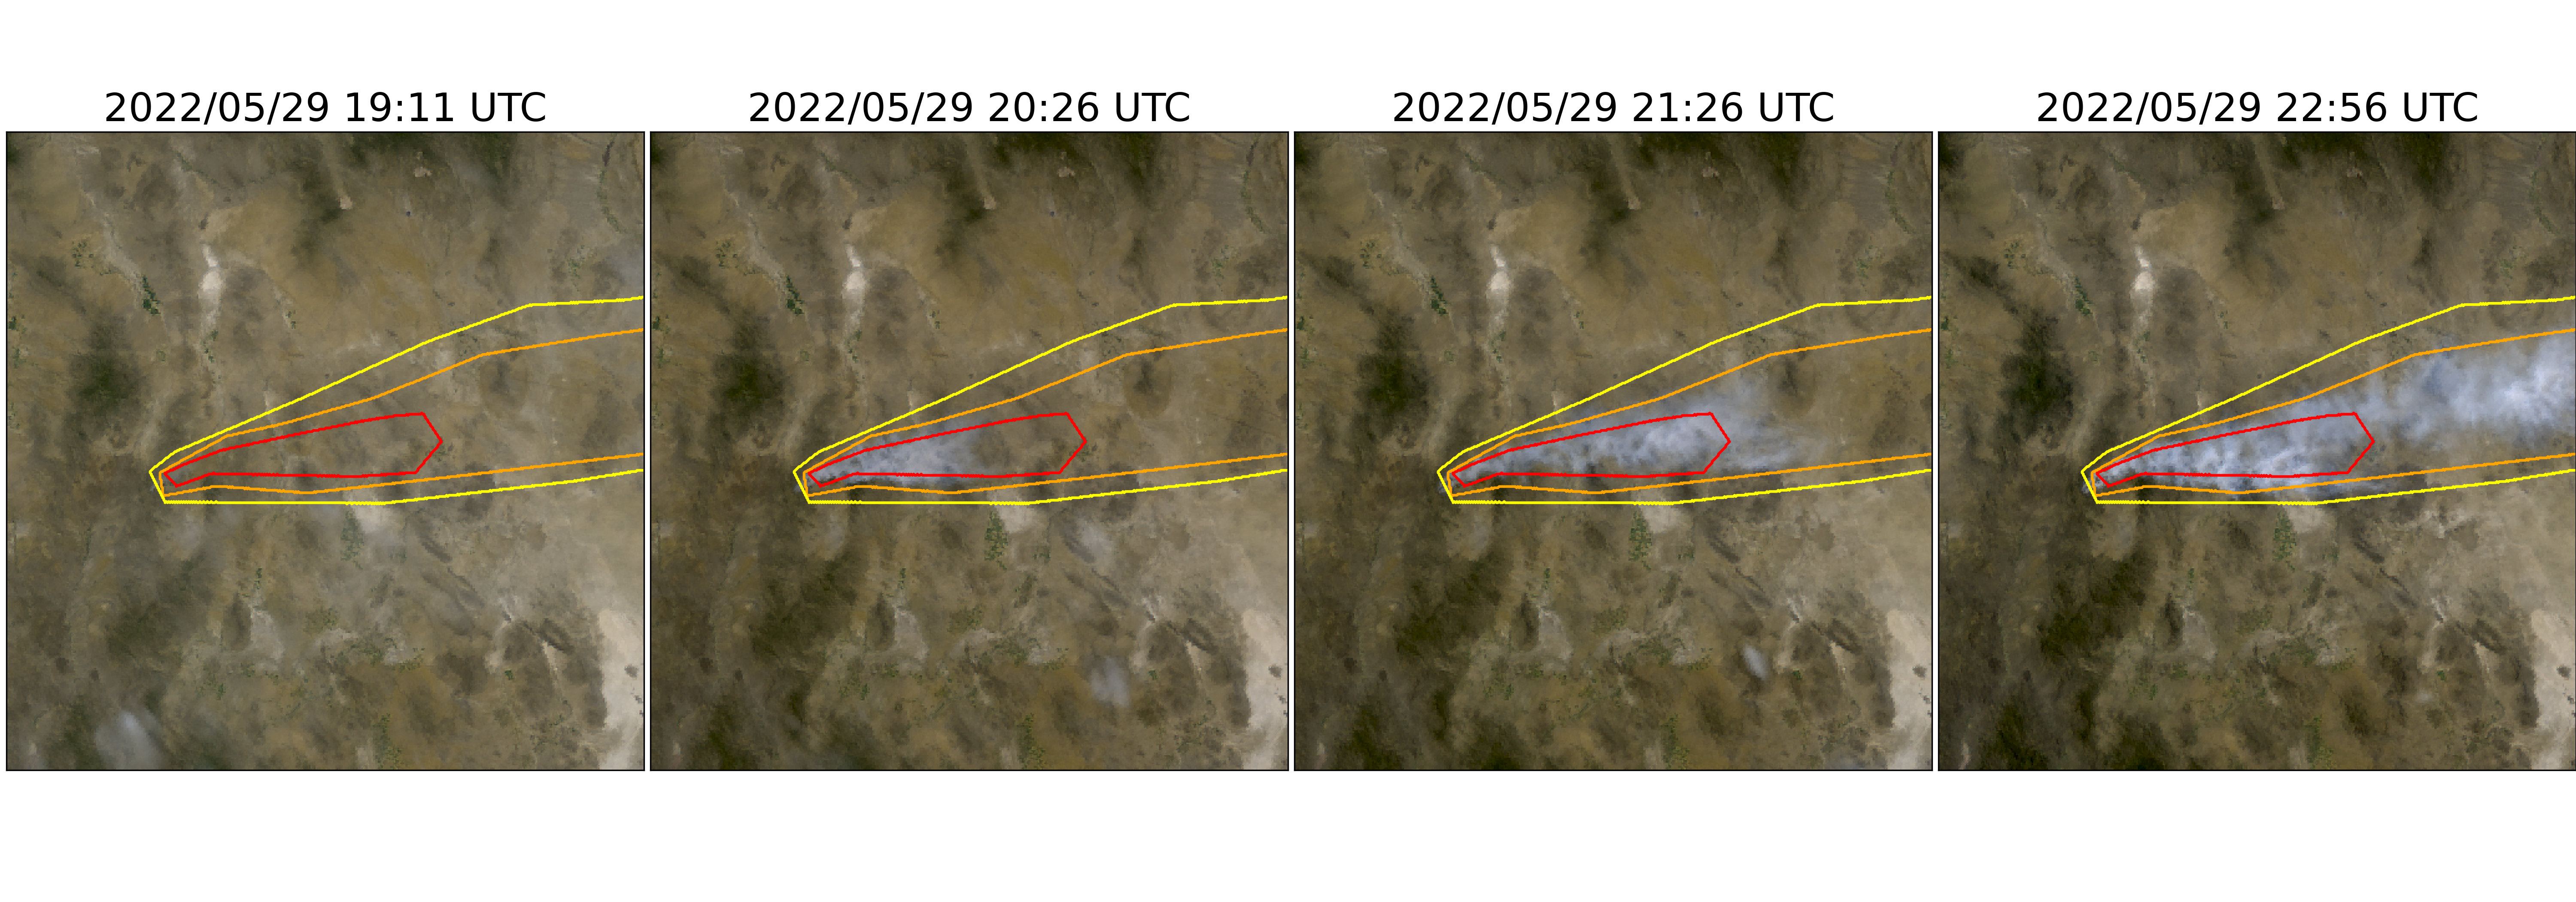
\includegraphics[width=13cm]{figures/timelapse.png}
    \caption{True color GOES-East imagery from May 2022, Southeast New Mexico (\(31^{\circ}\)N, \(100^{\circ}\)W) during the start of the Foster Fire. The red, orange and yellow lines represent the heavy, medium and low density HMS smoke annotations that span 19:10\textendash23:00 UTC.}
\end{figure}


\subsubsection*{Satellite Imagery} 

The GOES satellites are operated by NOAA in order to support meteorology research and forecasting for the United States. We use the latest operational satellites, GOES-16 (East), 17 and 18 (West) that each carry the ABI, that measure 16 bands between the visible and infrared wavelengths. In improvement to the GOES predecessors, imagery is collected every 5 minutes for the contiguous United States and every 10 minutes for the full disk. Using PyTroll, a Python framework for processing satellite data \cite{satpy}, we input bands 1-3 (Table \ref{rgb_bands}) to a GOES specific true color composite algorithm \cite{true_color} to develop a, 1km resolution, true color image representation, similar to what is seen by HMS analysts. As discussed in further detail in the next section, the highest signal-to-noise ratio will come from the smallest wavelengths of light, higher wavelengths have lower smoke signal and higher noise (figure \ref{bands}). For that reason, we only include the first 3 out of 16 available bands of data.

\begin{table}
    \caption{To create a true color image, we use the following bands from the ABI Level 1b CONUS (ABI-L1b-RadC) product.}\label{rgb_bands}
    \centering
        \begin{tabular}{ccccrrcrc}
            \toprule
            band & description & center wavelength ($\mathrm{\mu m}$) & spatial resolution (km)\\
            \midrule
            C01 &  blue visible & 0.47 & 1 \\
            C02 & red visible & 0.64 & 0.5 \\
            C03 & veggie near infrared & 0.865 & 1 \\
            \bottomrule
        \end{tabular}
\end{table}


\subsubsection*{Mie-Derived Dataset}

We used a physics-informed approach in selecting the initial GOES dataset, \(\mathcal{X}_M\), which we call the Mie-derived dataset, for training an initial parent model, \(f_{\circ}\), where if \(\mathcal{X}\) represents all the GOES imagery corresponding to the HMS smoke annotation time window, \(\mathcal{X}_M \subset \mathcal{X}\). Prior GOES ABI datasets for machine learning applications often include data from only one of the two GOES-series satellites, commonly opting for GOES-East \cite{smoke_goes}, \cite{wildfire_detect}, \cite{goes_conv}. Rather than using one satellite or the cumulative data from both GOES-West and GOES-East images, we select between one or the other based on the solar zenith angle. For smoke identification, this approach can achieve a much higher signal-to-noise than imaging the earth’s surface from an arbitrary angle. The elastic scattering of light is the primary mechanism to account for - while the atmosphere is composed of molecules with size \(<\)1nm, smoke particles can vary from 100 nm -- 10 \(\mu\)m in diameter, \(d\). The GOES ABI covers spectral bands from 0.47 \(\mu\)m -- 13.3 \(\mu\)m, so atmospheric and smoke particle sizes occupy two very different regimes with respect to the imaging wavelength \(\lambda\). In the extreme limit of \(\lambda \gg d\), the physics of scattering of light off a small sphere is captured by Rayleigh scattering. This process has two critical consequences: (1) the scattering cross section of light is strongly wavelength dependent (scaling with \(\lambda^{-4}\)), meaning that photons with wavelength closer to the ultraviolet are scattered more strongly than infrared photons. (2) the scattering cross section scales with an angular dependent cross section of \((1 + \cos^2 \theta)\). Scattered photons follow the emission distribution of a radiating dipole, scattering more strongly in the forward and backwards directions \((\theta = 0,\pi)\)than orthogonal to the direction of propagation \((\theta = \pi/2, 3\pi/2)\), see figure \ref{mei} for a Rayleigh scattering schematic.

%\begin{figure}
%    \centering
%    \includegraphics[width=10cm]{figures/scatter_regime.png}
%    \caption{Relationship between the size of a particle, the wavelength of light interacting with the particle and the type of scattering behavior induced by that interaction. The dotted lines represent rough estimates of the boundaries between the scattering regimes \cite{petty}. The gray area represents the range of particle radius relevant to smoke particulate matter.}\label{regime}
%\end{figure}

\begin{figure}
    \centering
    \includegraphics[width=10cm]{figures/mei.png}
    \caption{If the particle size is \(<\frac{1}{10}\) the wavelength of the interacting light, then the primary scattering will be Rayleigh. Mie scattering is the predominant scattering mechanism when the particle size is larger than the wavelength of light. This schematic demonstrates that when the sun is setting in the West, the Mie scattering will predominately forward scatter towards GOES-East.} \label{mei}
\end{figure}

The significance of these scalings is that the observer, or detector, will receive blue photons in most directions orthogonal to the source. Equivalently, photons traveling colinearly with line of sight to the emission source will mostly have wavelengths in the infrared band. In the converse regime of \(d > \lambda\), the elastic scattering of light against matter is modeled through Mie scattering. In comparison to Rayleigh scattering, Mie scattering is largely wavelength-independent and has a more complicated radiation pattern where the cross section has a maximal amplitude in the forward direction. An observer downstream of this scatterer will collect more photons than one positioned directly behind it. In the context of smoke identification, a sunrise or sunset will lead to a higher Mie scattered signal in GOES-West and GOES-East respectively, as shown with a smoke plume producing a stronger signal in GOES-East imagery near sunset in figure \ref{16_vs_17}.

\begin{figure}
    \centering
    \includegraphics[width=11cm]{figures/G16_v_G17.png}
    \caption{True color GOES-East (left) and GOES-West (right) imagery from April \(24^{th}\), 2022 in Durango, Mexico. The images were taken \(\sim0.5\) hours before sunset (01:43 UTC) for this geolocation and time of year.}\label{16_vs_17}
\end{figure}

Smoke identification therefore amounts to extracting a signal of \(d > \lambda\) photons from the \(\lambda \gg d\) background. Positioning a detector along line of sight to the scatterer will result in a higher signal from smoke particles (figure \ref{mei}). Filtering the imaged wavelength can enhance this signal; photons collected in the blue spectrum will have a naturally lower background along the line of sight to the illumination source do their high level of Rayleigh scattering as. Therefore, as demonstrated in figure \ref{bands}, this configuration results in the highest signal to noise imaging for smoke particles.

\begin{figure}
    \centering
    \includegraphics[width=9cm]{figures/GOES16_bands.png}
    \caption{Three bands of GOES-East data are the raw input to generate a true color image. These plots show variations in the signal-to-noise ratio for smoke detection in relation to the wavelength, \(\lambda\), of light being measured.}\label{bands}
\end{figure}

Based solely on these criteria, the optimal strategy would be to pull data from GOES-West right after sunrise and from GOES-East right before sunset. Another factor to consider is that the time when the sun is in optimal alignment with the satellite for smoke detection coincides with when solar zenith angle is maximized. Larger angles between the satellite and sun result in an increase in noise due to increased atmospheric interactions \cite{zen_angle}. This is shown in figure \ref{G17_sunrise}, while we optimize for smoke signal detection, due to the high solar zenith angle, we introduce atmospheric interaction noise that obfuscate the smoke signal. To reduce the noise from large solar zenith angles, if given multiple frames to choose from, we choose the image with the largest solar zenith angle that is \(<80^{\circ}\).



The resulting image selection process takes into account atmospheric properties and light scattering physics to generate an estimate of which singular satellite image within the analyst time-window could give the highest smoke signal-to-noise ratio. The resulting Mie-derived dataset, \(\mathcal{X}_M = \{X_M, Y\}\), was then used to train a model, \(f_{\circ}\), that would generate \(N\) pseudo-labels, \(y^*\), for every sample, where \(N\) is determined by how many images, taken at a 10 minute interval, fit within the analyst time-window for that sample. Chosen from the \(N\) images, \(x_p\) is the image with the highest alignment between the \(f_{\circ}\) prediction of smoke, \(y^*\), in the image and the HMS analysts' annotation \(y\).

\begin{figure}
    \centering
    \includegraphics[width=12cm]{figures/timelapse_G17_2.png}
    \caption{A smoke annotation projected onto GOES-West imagery from August 2022 that spans from 11:00 UTC to 15:00 UTC, sunrise on August 2nd, 2022 at coordinates (49°24'N, 115°29'W) was 12:15 UTC.}\label{G17_sunrise}
\end{figure}

\subsubsection*{Machine Learning Model} 

We implement a deep learning architecture that uses the encoder from EfficientNetV2 \cite{efficientnetv2} and a semantic segmentation classifier from the DeepLabV3 model \cite{deeplab}. Transfer learning has shown to reduce the time and resources needed to train a model by leveraging information from pre-trained models \cite{transfer}, \cite{transfer2}. We initialize the values of our model weights using the pre-trained values originally trained on the ImageNet dataset \cite{imgnet}, containing 1.2 million images and 1000 categories. Our model was developed using the Segmentation Models PyTorch package \cite{semantic} that was written as a high level API for implementing models for semantic segmentation problems. We input 256x256x3 snapshots of 1km resolution true color GOES imagery that contains smoke and output a 256x256x3 classification map that predicts if a pixel contains smoke and if so, what the density of that smoke is. As mentioned earlier, we apply the thermometer encoding shown in table \ref{therm} to encode the smoke densities and apply binary cross entropy as the loss function per density of smoke. 


The dataset, \(\mathcal{X}_M\), contained over 130,000 samples. To train \(f_{\circ}\), we split \(\mathcal{X}_M\) into training (118,691 samples), validation (8,335 samples) and testing (7,474 samples) datasets. Training data contains data from the years 2018, 2019, 2020, 2021 and 2023 while the data from 2022 is split into validation and testing sets by taking data from alternating 10 days of the year. In order to make sure we include the monthly variations in wildfire trends over a full year, we split 2022 data up by every 10 days. This allowed us to: (1) allocate an additional full year of data for the training set, (2) show yearlong trends in both the validation and testing sets and (3) keep the validation and testing datasets relatively independent from one another since only two out of every ten days of data will have adjacent days in validation and testing.

To determine which image out of the relevant imagery for the given time window best represents the analyst annotation, we implement a greedy algorithm by running \(f_{\circ}\) on each \(x\) to generate a pseudo-label, \(y^*\). The output of \(f_{\circ}\), \(y^*\), give predictions on if smoke is in the image, and if there is smoke, where the smoke is in that image and the density of that smoke. \(y^*\) serve as pseudo-labels for each density of smoke and are compared to the analyst annotations, \(y\). To compare \(y^*\) and \(y\), we calculate the IoU using the total set of pixels for \(y^*\) at that density of smoke and the entire set of pixels for \(y\) for a particular smoke density in each image as shown in equation \ref{overall_iou}. The image with the highest IoU score is chosen as the image, \(x_p\), that best represents the analyst smoke annotation, \(y\). Often used for pseudo-labeling, a confidence threshold value is defined to determine if a pseudo-label should to be included in a dataset \cite{conf_thresh}. We chose a confidence threshold that would include the sample, \(x_p\), in \(\mathcal{X}_{p}\) if the maximum overall IoU (equation \ref{overall_iou}) between \(y^*\) and \(y\) over all densities was over 0.01. 

\begin{equation} \label{overall_iou}
    IoU_{\text{overall}} = \frac{\sum\limits_{i=\text{light}}^{\text{heavy}}|y_{i}\cap y^*_{i}|}{\sum\limits_{i=\text{light}}^{\text{heavy}}|y_{i}|\cup|y^*_{i}|}
\end{equation}

Finally, we use \(\mathcal{X}_{p}\) to train an additional child model, \(f_c\). We use the same dataset split method and model setup but change \(\mathcal{X}_M\) to \(\mathcal{X}_{p}\) to train the child model. For training both \(f_c\) and \(f_p\) we train each model over 10 epochs using the Adam optimizer on a single Nvidia A100 GPU allocating 10GB of memory over 80 hours of allotted training time.

\section*{Results}

To interpret the performance of \(f_{\circ}\), we report the IoU metrics in table \ref{iou_results} that were computed by running \(f_{\circ}\) and \(f_c\) on \(\mathcal{X}_M\) and \(\mathcal{X}_{p}\). For each density, we calculate the IoU using the total set of pixels that \(f_{\circ}\) predicts as that density of smoke and the entire set of pixels labeled by the analyst as a particular smoke density over all imagery contained in the testing dataset. Additionally, we compute the overall IoU for all densities by first computing the number of pixels that intersect their corresponding density and divide that by the total number of pixels that make up the union of model predicted and analyst labeled smoke in the testing dataset.



\begin{table} 
    \caption{IoU results per density of smoke and over all densities using \(f_{\circ}\) and \(f_c\) with \(\mathcal{X}_M\) and \(\mathcal{X}_p\).}\label{iou_results}
    \centering
    \begin{tabular}{lcc|cc}
        \toprule
        \multicolumn{1}{c}{} & \multicolumn{2}{c}{\(f_{\circ}\)} & \multicolumn{2}{c}{\(f_c\)}\\
        \midrule
        \multicolumn{1}{c}{} & \(\mathcal{X}_M\) & \(\mathcal{X}_{p}\) & \(\mathcal{X}_M\) & \(\mathcal{X}_{p}\) \\
        \midrule
        Light  & 0.394 &  0.551 & 0.437 &  0.583 \\
        Medium & 0.283 &  0.392 & 0.345 &  0.431 \\
        Heavy  & 0.233 &  0.290 & 0.275 &  0.332 \\
        Overall & 0.365 &  0.510 & 0.412 &  0.539 \\
        \bottomrule
    \end{tabular}
\end{table}

\begin{figure}
    \centering
    %\includegraphics[width=12cm]{figures/ML_better_than_Mie_2.png}
    \includegraphics[width=14cm]{figures/D_m_vs_D_pl.png}
    \caption{GOES-West imagery showing smoke on June 8th, 2022 in Alaska where, at this geolocation, daylight was between 12:43-7:53 UTC. The HMS smoke annotations displayed span from 18:50 to 23:50 UTC. a) shows the imagery that was selected using the Mie-derived data selection process b) shows the image that had the highest IoU score between the \(f_{\circ}\) generated pseudo-label and the analyst annotation.}\label{ml_vs_mei}
\end{figure}

An illustration of a pseudo-label picked image better representing the analyst annotation when compared to the Mie-derived image selection is evident in Figure \ref{ml_vs_mei}, where the heavy density smoke IoU increases from 0.01 to 0.59. The analyst annotation for these densities cover 5 hours of imagery, the Mie-derived selection optimizes for the image closest to sunrise while the pseudo-label image selection chooses the image with the highest overlap between the pseudo-label and the analyst annotation. 

\section{Limitations}

One of the concerns that comes with using pseudo-labeling methods is that you can perpetuate biases from the parent model into subsequent child models. Due to the increase in detectable forward scattered light off smoke particular matter, we expect the model to have a bias towards producing a higher success rate for smoke detection at larger solar zenith angles. Another concern is the possibility of a data leak between the adjacent days every 10 days for validation and testing set. Finally, the original HMS dataset is not split by type of fire and includes a large portion of small, controlled burns. This can be a limitation to consider if the dataset is being used to detect large wildfires. All these limitations are discussed and analyzed further in the Appendix. 

\section{Conclusion}

In this study, we have refined an existing dataset originally curated by NOAA's HMS team, transforming it from a many-to-one imagery-to-annotation format to a more succinct, one-to-one satellite image-to-annotation dataset. The initial HMS dataset primarily provided a general approximation of where smoke had been present for a given time window, though it did not guarantee the actual existence of smoke in the labeled pixels during the given times. Our goal was to create a dataset that could be used, along with additional applications, to train a model to detect wildfire smoke in real-time on an image-by-image level. The Mie-derived dataset selection process determines that if smoke is present, what timestamp within the analyst time window would the give the highest smoke signal-to-noise ratio. While optimizing for being able to detect smoke, if it is present, the Mie-dataset selection had no metric to determine if the smoke was effectually present in the selected image. Since many of the images within the HMS time-window either contained no smoke at all or the smoke was not contained within the geospatial bounds of the annotations, the Mie-derived dataset contained a large number of mislabeled samples. Discrepancies between data and labels can be detrimental towards the model's capacity to improve on feature representations in the target domain. During model training, the penalization of accurate predictions can inadvertently introduce biases towards misclassifying noise as meaningful signal. 

To improve the dataset's capacity to accurately represent wildfire smoke plumes, we train a parent machine learning model, \(f_{\circ}\), using the Mie-derived dataset, \(\mathcal{X}_M\), and run it on the relevant satellite images within the time-frame. The image with the maximum IoU score between the model's smoke predictions, or pseudo-label, and the analyst smoke annotations are used to create the pseudo-label generated dataset, \(\mathcal{X}_{p}\). We then train a child model, \(f_c\), using \(\mathcal{X}_{p}\) and test \(f_{\circ}\) and \(f_c\) on both the 2022 testing sets from \(\mathcal{X}_{M}\) and \(\mathcal{X}_{p}\). The results reported in table \ref{iou_results} suggest that \(\mathcal{X}_{p}\) was able to train a better performing model, \(f_c\), that gave higher IoU metrics on both dataset's testing sets in comparison to the original parent model, \(f_{\circ}\).

The result of this study is a representative dataset that can be used to train machine learning models for various wildfire smoke applications. A future goal is to produce a robust and reliable machine learning based approach for detecting wildfires using satellite imagery. That information can be used for wildfire monitoring and as data provided to public health officials for air quality assessments. On a broader scale, we show how pseudo-labeling can be used to optimize a dataset when the resolution for the data and corresponding labels do not match. This could be useful in similar applications involving time-series/video data with a singular label where the data can be compressed while still remaining representative of the label. 

\section{Acknowledgments and Disclosure of Funding}

This research was supported in part by NOAA cooperative agreement NA22OAR4320151, for the Cooperative Institute for Earth System Research and Data Science (CIESRDS). We thank Wilfrid Schroeder and the Hazard Mapping Systems team for giving guidance on how they created their smoke plume dataset. This work utilized the Alpine high performance computing resource at the University of Colorado Boulder. Alpine is jointly funded by the University of Colorado Boulder, the University of Colorado Anschutz, Colorado State University, and the National Science Foundation (award 2201538). The statements, findings, conclusions, and recommendations are those of the author(s) and do not necessarily reflect the views of NOAA or the U.S. Department of Commerce. 

\bibliography{references}

\appendix

\section{Appendix}



\subsection{Original Data and Software Licenses}
The HMS Smoke product does not have a license attached to it. For GOES imagery, NOAA states "There are no restrictions on the use of this data" and does not provide a license. Pytroll is distributed under the GNU General Public License v3.0 license while Segmentation Models Pytorch is distributed under the MIT License.


\subsection{Statistical Visualizations for SmokeViz Dataset}

Figures \ref{count_per_yr}, \ref{count_per_month}, \ref{count_per_state}, \ref{count_per_country} provide some statistical analysis on \(\mathcal{X}_p\). As seen in figure \ref{count_per_yr}, we see the highest number of samples for the year 2020 that showed a high volume of available annotations that year likely due to the large number of wildfires \cite{fires2020} during 2020. The peak for number of samples shown in figure \ref{count_per_month} is March and April, coming right before the typical wildfire season that usually goes from late Spring through Fall. This may be due to the increase in prescribed agricultural burns before plants emerge from winter dormancy \cite{ag_fire}. The HMS analysts do not have a way of distinguishing between planned or uncontrolled fire, so many of the annotations represent small agricultural burns along with wildfires. 

As shown in figure \ref{count_per_state}, the states with the highest number of samples are California, Georgia and Florida. The high frequency in fires in the Southeast may be due to the aforemetioned prescirbed agricultural burns. Analysts are looking not only at the United States, but also Canada and Mexico, figure \ref{count_per_country} shows a breakdown of the number of samples that originate from each country.


\begin{figure}
    \centering
    \includegraphics[width=8cm]{stat_figs/sample_count_per_yr.png}
    \caption{Sample count per year}\label{sample_count_per_yr}\label{count_per_yr}
\end{figure}

\begin{figure}
    \centering
    \includegraphics[width=8cm]{stat_figs/sample_count_per_month.png}
    \caption{Sample count per month.}\label{sample_count_per_month}\label{count_per_month}
\end{figure}

\begin{figure}
    \centering
    \includegraphics[width=10cm]{stat_figs/sample_count_per_state.png}
    \caption{Sample count per US state.}\label{count_per_state}
\end{figure}

\begin{figure}
    \centering
    \includegraphics[width=10cm]{stat_figs/sample_count_per_country.png}
    \caption{Sample count per North American country.}\label{count_per_country}
\end{figure}


\subsection{Model Performance Analysis}

In order to get a better understanding of the dataset, we use the deep learning models to analyze certain data characteristics. Figure \ref{iou_per_month} shows variations in overall IoU values running \(f_{\circ}\) on the \(\mathcal{X}_p\) test set data. The highest IoU are during the typical wildfire season and outside the typical window for prescribed agricultural burns. 

\begin{figure}
    \centering
    \includegraphics[width=8cm]{stat_figs/IoU_per_month.png}
    \caption{IoU between \(f_{c}\) predictions and analyst annotations per month for \(\mathcal{X}_p\) test set.}\label{iou_per_month}
\end{figure}


We report on how many samples come from each satellite in table \ref{sample_count_sat}, along with the \(\mathcal{X}_p\) test set IoU in comparison to the HMS analyst annotations. While GOES-EAST provides over triple the number of training samples, \(f_c\) performs better on GOES-WEST samples out of the test set. The signal observed by a single satellite vary diurnally and annually in the amount of atmospheric noise and solar radiation. In turn, if provided with enough samples, this could create a more robust and generalizable model to the extent of being able to perform well on two different sensors with varying calibrations and line of sights. 

As mentioned in the limitations, there may have been a bias introduced towards correctly classifying imagery close to sunrise or sunset. This bias may not only be introduced by our Mie-derived dataset that was used to train \(f_{\circ}\), but also in the original HMS annotations. The configuration of the sun, smoke and satellite give the highest signal-to-noise ratio at the times near the sunrise and sunset, making smoke more easily observable. In contrast, the diurnal variations of wildfires cause the fire radiative power to be highest around solar noon \cite{diurnal}. Table \ref{two_hr_iou} shows how the IoU between \(f_c\) predictions and analyst annotations for the test data from either \(\mathcal{X}_M\) or \(\mathcal{X}_p\) are not significantly affected by being within 2 hours to sunrise/sunset. The main difference we see from table \ref{two_hr_iou} is the split of closer to daylight boundaries is shifted towards midday between \(\mathcal{X}_M\) to \(\mathcal{X}_p\). This is because, for \(\mathcal{X}_p\), we are choosing the imagery with the best overlap to the analyst product rather than the image from \(\mathcal{X}_M\) that optimized for highest possible signal-to-noise ratio if given constant signal.


In order to observe geographical regional variations we create quadrants, Northwest (NW), Southwest (SW), Northeast (NE) and Southeast (SE) in relation to the midpoint (40, -100) and show the sample distribution and model performance for each region in table \ref{quad}. The table shows the worst \(f_c\) performance in the SE quadrant despite representing this largest fraction of the training data. This is likely due to the large number of aforementioned prescribed burns in that area. If the goal of the dataset is to be used to train a model to detect and monitor large wildfires, a weakness in the dataset would be that it likely consists of a lot more small, controlled agricultural burns that aren't representative of the intended task. 

A weakness in the dataset split for 2022 validation and testing sets is that there are adjacent days between the rotating 10 day splits. This is a weakness because wildfires often last more than one day, smoke from the same fires are likely to leak between the datasets. The choice to split the dataset every 10 days was a trade off between being able to keep another day for training and keeping the validation and test set completely independent. Another consideration for the choice was that we expect the diurnal variations in smoke characteristics to vary largely enough at either ends of the nocturnal stagnations in fire activity \cite{night}. The scope of this paper was to use the deep learning models as a way of optimizing the dataset and comparing the datasets against each other. While the data leak is not likely to have high consequences for this particular application (as suggested in table \ref{adjacent}), we encourage users of SmokeViz to split validation and test sets so that they are completely independent, especially as new years of data are added. 

\begin{table}
    \caption{Sample count along with variations in \(f_c\) performance depending on which GOES satellite data is used.}
  \label{sample_count_sat}
  \centering
  \begin{tabular}{llll}
    \toprule
    Satellite & Test IoU & \(\mathcal{X}_p\) Test Samples & \(\mathcal{X}_p\) Samples \\
    \midrule
    GOES-WEST & 0.645 & 1827 & 30640   \\
    GOES-EAST & 0.483 & 5647 & 119040 \\
    \bottomrule
  \end{tabular}
\end{table}


\begin{table}
    \caption{Variations in \(f_c\) performance depending on temporal proximity to sunrise or sunset.}
  \label{two_hr_iou}
  \centering
  \begin{tabular}{lllll}
    \toprule
    Time difference & \(\mathcal{X}_M\) Test Set IoU & \(\mathcal{X}_p\) Test Set IoU & \(\mathcal{X}_M\) Test Samples & \(\mathcal{X}_p\) Test Samples \\ 
    \midrule
    <2 hours & 0.412 & 0.546 & 3923 (63\%) & 3436 (46\%)\\
    >2 hours & 0.411 & 0.538 & 2280 (37\%) &   4038 (54\%) \\
    \bottomrule
  \end{tabular}
\end{table}


\begin{table}
    \caption{Along with sample count we show variations in \(f_{c}\) performance depending on quadrant.}
  \label{quad}
  \centering
  \begin{tabular}{llll}
    \toprule
    Quadrant & \(\mathcal{X}_p\) Test IoU & \(\mathcal{X}_p\) Test Samples & \(\mathcal{X}_p\) Samples \\
    \midrule
    NW & 0.5932 & 1425  &  23335 \\
    SW & 0.6094 & 1131  &  26577 \\
    NE & 0.4726 & 252   &  8392 \\
    SE & 0.4706 & 4666  &  76130 \\
    \bottomrule
  \end{tabular}
\end{table}

\begin{table}
    \caption{Comparison of the IoU and loss between the full \(\mathcal{X}_p\) test set and the \(\mathcal{X}_p\) test set with adjacent days between the validation and test set removed.}
  \label{adjacent}
  \centering
  \begin{tabular}{lll}
    \toprule
    \(\mathcal{X}_p\) Test Set &   Overall IoU   &  Testing Loss \\
    \midrule
    full test set  & 0.539 &   0.870 \\
    adjacent days removed &  0.547 &  0.895 \\
    \bottomrule
  \end{tabular}
\end{table}

\subsection{Machine Learning Reproducibility}

The models presented in this paper are not optimized for performance, but are intended to create sufficient pseudo-labels to develop the SmokeViz dataset and then compare the performance of SmokeViz against the original dataset. We did not perform any experimentation for deciding on architecture or hyperparameters but did make educated decisions. We chose DeepLabV3+ because smoke varies in scale and the DeepLabV3+ backbone uses a atrous spatial pyramid pooling module that allows for varying scales of the same type of object. We use the Adam optimizer that will adapt the learning rate during training and is suited for problems with large amounts of data. Batch size was chosen due to the necessity to run the model on limited resources. 

\begin{table}
    \caption{Hyperparameters used to create \(f_{\circ}\) and \(f_{c}\).}
  \label{hyper}
  \centering
  \begin{tabular}{ll}
    \toprule
    parameter & value \\ 
    \midrule
    epochs & 10 \\
    learning rate & 1e-2 \\
    batch size & 32 \\
    optimizer & Adam \\
    \bottomrule
  \end{tabular}
\end{table}





\newpage
\section*{NeurIPS Paper Checklist}

\begin{enumerate}

\item {\bf Claims}
    \item[] Question: Do the main claims made in the abstract and introduction accurately reflect the paper's contributions and scope?
    \item[] Answer: \answerYes{} % Replace by \answerYes{}, \answerNo{}, or \answerNA{}.
    \item[] Justification: The claims of using pseudolabels to create a more robust dataset is reflected in the paper's contributions. 
    \item[] Guidelines:
    \begin{itemize}
        \item The answer NA means that the abstract and introduction do not include the claims made in the paper.
        \item The abstract and/or introduction should clearly state the claims made, including the contributions made in the paper and important assumptions and limitations. A No or NA answer to this question will not be perceived well by the reviewers. 
        \item The claims made should match theoretical and experimental results, and reflect how much the results can be expected to generalize to other settings. 
        \item It is fine to include aspirational goals as motivation as long as it is clear that these goals are not attained by the paper. 
    \end{itemize}

\item {\bf Limitations}
    \item[] Question: Does the paper discuss the limitations of the work performed by the authors?
    \item[] Answer: \answerYes{} % Replace by \answerYes{}, \answerNo{}, or \answerNA{}.
    \item[] Justification: We address limitations of the dataset.
    \item[] Guidelines:
    \begin{itemize}
        \item The answer NA means that the paper has no limitation while the answer No means that the paper has limitations, but those are not discussed in the paper. 
        \item The authors are encouraged to create a separate "Limitations" section in their paper.
        \item The paper should point out any strong assumptions and how robust the results are to violations of these assumptions (e.g., independence assumptions, noiseless settings, model well-specification, asymptotic approximations only holding locally). The authors should reflect on how these assumptions might be violated in practice and what the implications would be.
        \item The authors should reflect on the scope of the claims made, e.g., if the approach was only tested on a few datasets or with a few runs. In general, empirical results often depend on implicit assumptions, which should be articulated.
        \item The authors should reflect on the factors that influence the performance of the approach. For example, a facial recognition algorithm may perform poorly when image resolution is low or images are taken in low lighting. Or a speech-to-text system might not be used reliably to provide closed captions for online lectures because it fails to handle technical jargon.
        \item The authors should discuss the computational efficiency of the proposed algorithms and how they scale with dataset size.
        \item If applicable, the authors should discuss possible limitations of their approach to address problems of privacy and fairness.
        \item While the authors might fear that complete honesty about limitations might be used by reviewers as grounds for rejection, a worse outcome might be that reviewers discover limitations that aren't acknowledged in the paper. The authors should use their best judgment and recognize that individual actions in favor of transparency play an important role in developing norms that preserve the integrity of the community. Reviewers will be specifically instructed to not penalize honesty concerning limitations.
    \end{itemize}

\item {\bf Theory Assumptions and Proofs}
    \item[] Question: For each theoretical result, does the paper provide the full set of assumptions and a complete (and correct) proof?
    \item[] Answer: \answerNA{} % Replace by \answerYes{}, \answerNo{}, or \answerNA{}.
    \item[] Justification: No theoretical results are presented. 
    \item[] Guidelines:
    \begin{itemize}
        \item The answer NA means that the paper does not include theoretical results. 
        \item All the theorems, formulas, and proofs in the paper should be numbered and cross-referenced.
        \item All assumptions should be clearly stated or referenced in the statement of any theorems.
        \item The proofs can either appear in the main paper or the supplemental material, but if they appear in the supplemental material, the authors are encouraged to provide a short proof sketch to provide intuition. 
        \item Inversely, any informal proof provided in the core of the paper should be complemented by formal proofs provided in appendix or supplemental material.
        \item Theorems and Lemmas that the proof relies upon should be properly referenced. 
    \end{itemize}

    \item {\bf Experimental Result Reproducibility}
    \item[] Question: Does the paper fully disclose all the information needed to reproduce the main experimental results of the paper to the extent that it affects the main claims and/or conclusions of the paper (regardless of whether the code and data are provided or not)?
    \item[] Answer: \answerYes{} % Replace by \answerYes{}, \answerNo{}, or \answerNA{}.
    \item[] Justification: We provide the code to create the datasets along with the final dataset hosted on AWS by NOAA.
    \item[] Guidelines:
    \begin{itemize}
        \item The answer NA means that the paper does not include experiments.
        \item If the paper includes experiments, a No answer to this question will not be perceived well by the reviewers: Making the paper reproducible is important, regardless of whether the code and data are provided or not.
        \item If the contribution is a dataset and/or model, the authors should describe the steps taken to make their results reproducible or verifiable. 
        \item Depending on the contribution, reproducibility can be accomplished in various ways. For example, if the contribution is a novel architecture, describing the architecture fully might suffice, or if the contribution is a specific model and empirical evaluation, it may be necessary to either make it possible for others to replicate the model with the same dataset, or provide access to the model. In general. releasing code and data is often one good way to accomplish this, but reproducibility can also be provided via detailed instructions for how to replicate the results, access to a hosted model (e.g., in the case of a large language model), releasing of a model checkpoint, or other means that are appropriate to the research performed.
        \item While NeurIPS does not require releasing code, the conference does require all submissions to provide some reasonable avenue for reproducibility, which may depend on the nature of the contribution. For example
        \begin{enumerate}
            \item If the contribution is primarily a new algorithm, the paper should make it clear how to reproduce that algorithm.
            \item If the contribution is primarily a new model architecture, the paper should describe the architecture clearly and fully.
            \item If the contribution is a new model (e.g., a large language model), then there should either be a way to access this model for reproducing the results or a way to reproduce the model (e.g., with an open-source dataset or instructions for how to construct the dataset).
            \item We recognize that reproducibility may be tricky in some cases, in which case authors are welcome to describe the particular way they provide for reproducibility. In the case of closed-source models, it may be that access to the model is limited in some way (e.g., to registered users), but it should be possible for other researchers to have some path to reproducing or verifying the results.
        \end{enumerate}
    \end{itemize}


\item {\bf Open access to data and code}
    \item[] Question: Does the paper provide open access to the data and code, with sufficient instructions to faithfully reproduce the main experimental results, as described in supplemental material?
    \item[] Answer: \answerYes{} % Replace by \answerYes{}, \answerNo{}, or \answerNA{}.
    \item[] Justification: Pseudo-labeled derived dataset is released along with code to recreate it. 
    \item[] Guidelines:
    \begin{itemize}
        \item The answer NA means that paper does not include experiments requiring code.
        \item Please see the NeurIPS code and data submission guidelines (\url{https://nips.cc/public/guides/CodeSubmissionPolicy}) for more details.
        \item While we encourage the release of code and data, we understand that this might not be possible, so “No” is an acceptable answer. Papers cannot be rejected simply for not including code, unless this is central to the contribution (e.g., for a new open-source benchmark).
        \item The instructions should contain the exact command and environment needed to run to reproduce the results. See the NeurIPS code and data submission guidelines (\url{https://nips.cc/public/guides/CodeSubmissionPolicy}) for more details.
        \item The authors should provide instructions on data access and preparation, including how to access the raw data, preprocessed data, intermediate data, and generated data, etc.
        \item The authors should provide scripts to reproduce all experimental results for the new proposed method and baselines. If only a subset of experiments are reproducible, they should state which ones are omitted from the script and why.
        \item At submission time, to preserve anonymity, the authors should release anonymized versions (if applicable).
        \item Providing as much information as possible in supplemental material (appended to the paper) is recommended, but including URLs to data and code is permitted.
    \end{itemize}


\item {\bf Experimental Setting/Details}
    \item[] Question: Does the paper specify all the training and test details (e.g., data splits, hyperparameters, how they were chosen, type of optimizer, etc.) necessary to understand the results?
    \item[] Answer: \answerYes{} % Replace by \answerYes{}, \answerNo{}, or \answerNA{}.
    \item[] Justification: Dataset splits, hyperparameters, optimizer are specified.
    \item[] Guidelines:
    \begin{itemize}
        \item The answer NA means that the paper does not include experiments.
        \item The experimental setting should be presented in the core of the paper to a level of detail that is necessary to appreciate the results and make sense of them.
        \item The full details can be provided either with the code, in appendix, or as supplemental material.
    \end{itemize}

\item {\bf Experiment Statistical Significance}
    \item[] Question: Does the paper report error bars suitably and correctly defined or other appropriate information about the statistical significance of the experiments?
    \item[] Answer: \answerNo{} % Replace by \answerYes{}, \answerNo{}, or \answerNA{}.
    \item[] Justification: The results are represented in by the intersection over union values, there are no error bars.
    \item[] Guidelines:
    \begin{itemize}
        \item The answer NA means that the paper does not include experiments.
        \item The authors should answer "Yes" if the results are accompanied by error bars, confidence intervals, or statistical significance tests, at least for the experiments that support the main claims of the paper.
        \item The factors of variability that the error bars are capturing should be clearly stated (for example, train/test split, initialization, random drawing of some parameter, or overall run with given experimental conditions).
        \item The method for calculating the error bars should be explained (closed form formula, call to a library function, bootstrap, etc.)
        \item The assumptions made should be given (e.g., Normally distributed errors).
        \item It should be clear whether the error bar is the standard deviation or the standard error of the mean.
        \item It is OK to report 1-sigma error bars, but one should state it. The authors should preferably report a 2-sigma error bar than state that they have a 96\% CI, if the hypothesis of Normality of errors is not verified.
        \item For asymmetric distributions, the authors should be careful not to show in tables or figures symmetric error bars that would yield results that are out of range (e.g. negative error rates).
        \item If error bars are reported in tables or plots, The authors should explain in the text how they were calculated and reference the corresponding figures or tables in the text.
    \end{itemize}

\item {\bf Experiments Compute Resources}
    \item[] Question: For each experiment, does the paper provide sufficient information on the computer resources (type of compute workers, memory, time of execution) needed to reproduce the experiments?
    \item[] Answer: \answerYes{} % Replace by \answerYes{}, \answerNo{}, or \answerNA{}.
    \item[] Justification: We mention the A100 GPU, 10GB of memory and 80 hours of run time. 
    \item[] Guidelines:
    \begin{itemize}
        \item The answer NA means that the paper does not include experiments.
        \item The paper should indicate the type of compute workers CPU or GPU, internal cluster, or cloud provider, including relevant memory and storage.
        \item The paper should provide the amount of compute required for each of the individual experimental runs as well as estimate the total compute. 
        \item The paper should disclose whether the full research project required more compute than the experiments reported in the paper (e.g., preliminary or failed experiments that didn't make it into the paper). 
    \end{itemize}
    
\item {\bf Code Of Ethics}
    \item[] Question: Does the research conducted in the paper conform, in every respect, with the NeurIPS Code of Ethics \url{https://neurips.cc/public/EthicsGuidelines}?
    \item[] Answer: \answerYes{} % Replace by \answerYes{}, \answerNo{}, or \answerNA{}.
    \item[] Justification: There are no conflicts between the research and the NeurIPS Code of Ethics.
    \item[] Guidelines:
    \begin{itemize}
        \item The answer NA means that the authors have not reviewed the NeurIPS Code of Ethics.
        \item If the authors answer No, they should explain the special circumstances that require a deviation from the Code of Ethics.
        \item The authors should make sure to preserve anonymity (e.g., if there is a special consideration due to laws or regulations in their jurisdiction).
    \end{itemize}


\item {\bf Broader Impacts}
    \item[] Question: Does the paper discuss both potential positive societal impacts and negative societal impacts of the work performed?
    \item[] Answer: \answerYes{} % Replace by \answerYes{}, \answerNo{}, or \answerNA{}.
    \item[] Justification: There are no negative, but there are positive that are mentioned in the paper such as better tools for public health decision making. 
    \item[] Guidelines:
    \begin{itemize}
        \item The answer NA means that there is no societal impact of the work performed.
        \item If the authors answer NA or No, they should explain why their work has no societal impact or why the paper does not address societal impact.
        \item Examples of negative societal impacts include potential malicious or unintended uses (e.g., disinformation, generating fake profiles, surveillance), fairness considerations (e.g., deployment of technologies that could make decisions that unfairly impact specific groups), privacy considerations, and security considerations.
        \item The conference expects that many papers will be foundational research and not tied to particular applications, let alone deployments. However, if there is a direct path to any negative applications, the authors should point it out. For example, it is legitimate to point out that an improvement in the quality of generative models could be used to generate deepfakes for disinformation. On the other hand, it is not needed to point out that a generic algorithm for optimizing neural networks could enable people to train models that generate Deepfakes faster.
        \item The authors should consider possible harms that could arise when the technology is being used as intended and functioning correctly, harms that could arise when the technology is being used as intended but gives incorrect results, and harms following from (intentional or unintentional) misuse of the technology.
        \item If there are negative societal impacts, the authors could also discuss possible mitigation strategies (e.g., gated release of models, providing defenses in addition to attacks, mechanisms for monitoring misuse, mechanisms to monitor how a system learns from feedback over time, improving the efficiency and accessibility of ML).
    \end{itemize}
    
\item {\bf Safeguards}
    \item[] Question: Does the paper describe safeguards that have been put in place for responsible release of data or models that have a high risk for misuse (e.g., pretrained language models, image generators, or scraped datasets)?
    \item[] Answer: \answerNA{} % Replace by \answerYes{}, \answerNo{}, or \answerNA{}.
    \item[] Justification: There are no risks for misuse. 
    \item[] Guidelines:
    \begin{itemize}
        \item The answer NA means that the paper poses no such risks.
        \item Released models that have a high risk for misuse or dual-use should be released with necessary safeguards to allow for controlled use of the model, for example by requiring that users adhere to usage guidelines or restrictions to access the model or implementing safety filters. 
        \item Datasets that have been scraped from the Internet could pose safety risks. The authors should describe how they avoided releasing unsafe images.
        \item We recognize that providing effective safeguards is challenging, and many papers do not require this, but we encourage authors to take this into account and make a best faith effort.
    \end{itemize}

\item {\bf Licenses for existing assets}
    \item[] Question: Are the creators or original owners of assets (e.g., code, data, models), used in the paper, properly credited and are the license and terms of use explicitly mentioned and properly respected?
    \item[] Answer: \answerYes{} % Replace by \answerYes{}, \answerNo{}, or \answerNA{}.
    \item[] Justification: The raw NOAA datasets used to create SmokeViz do not have licenses while the python packages used do, we list these in the appendix.
    \item[] Guidelines:
    \begin{itemize}
        \item The answer NA means that the paper does not use existing assets.
        \item The authors should cite the original paper that produced the code package or dataset.
        \item The authors should state which version of the asset is used and, if possible, include a URL.
        \item The name of the license (e.g., CC-BY 4.0) should be included for each asset.
        \item For scraped data from a particular source (e.g., website), the copyright and terms of service of that source should be provided.
        \item If assets are released, the license, copyright information, and terms of use in the package should be provided. For popular datasets, \url{paperswithcode.com/datasets} has curated licenses for some datasets. Their licensing guide can help determine the license of a dataset.
        \item For existing datasets that are re-packaged, both the original license and the license of the derived asset (if it has changed) should be provided.
        \item If this information is not available online, the authors are encouraged to reach out to the asset's creators.
    \end{itemize}

\item {\bf New Assets}
    \item[] Question: Are new assets introduced in the paper well documented and is the documentation provided alongside the assets?
    \item[] Answer: \answerYes{} % Replace by \answerYes{}, \answerNo{}, or \answerNA{}.
    \item[] Justification: The dataset, supporting code and user-friendly Notebooks to play with the dataset/model all support the assets accessibility. 
    \item[] Guidelines:
    \begin{itemize}
        \item The answer NA means that the paper does not release new assets.
        \item Researchers should communicate the details of the dataset/code/model as part of their submissions via structured templates. This includes details about training, license, limitations, etc. 
        \item The paper should discuss whether and how consent was obtained from people whose asset is used.
        \item At submission time, remember to anonymize your assets (if applicable). You can either create an anonymized URL or include an anonymized zip file.
    \end{itemize}

\item {\bf Crowdsourcing and Research with Human Subjects}
    \item[] Question: For crowdsourcing experiments and research with human subjects, does the paper include the full text of instructions given to participants and screenshots, if applicable, as well as details about compensation (if any)? 
    \item[] Answer: \answerNA{} % Replace by \answerYes{}, \answerNo{}, or \answerNA{}.
    \item[] Justification: The paper does not involve crowdsourcing nor research with human subjects. 
    \item[] Guidelines:
    \begin{itemize}
        \item The answer NA means that the paper does not involve crowdsourcing nor research with human subjects.
        \item Including this information in the supplemental material is fine, but if the main contribution of the paper involves human subjects, then as much detail as possible should be included in the main paper. 
        \item According to the NeurIPS Code of Ethics, workers involved in data collection, curation, or other labor should be paid at least the minimum wage in the country of the data collector. 
    \end{itemize}

\item {\bf Institutional Review Board (IRB) Approvals or Equivalent for Research with Human Subjects}
    \item[] Question: Does the paper describe potential risks incurred by study participants, whether such risks were disclosed to the subjects, and whether Institutional Review Board (IRB) approvals (or an equivalent approval/review based on the requirements of your country or institution) were obtained?
    \item[] Answer: \answerNA{} % Replace by \answerYes{}, \answerNo{}, or \answerNA{}.
    \item[] Justification: The paper does not involve crowdsourcing nor research with human subjects.
    \item[] Guidelines:
    \begin{itemize}
        \item The answer NA means that the paper does not involve crowdsourcing nor research with human subjects.
        \item Depending on the country in which research is conducted, IRB approval (or equivalent) may be required for any human subjects research. If you obtained IRB approval, you should clearly state this in the paper. 
        \item We recognize that the procedures for this may vary significantly between institutions and locations, and we expect authors to adhere to the NeurIPS Code of Ethics and the guidelines for their institution. 
        \item For initial submissions, do not include any information that would break anonymity (if applicable), such as the institution conducting the review.
    \end{itemize}

\end{enumerate}


\end{document}
